\documentclass[12pt,a4paper,danish,oneside,openany]{memoir} 
% Skabelon af DTU's LaTeX support gruppe, v20090423

\usepackage[utf8]{inputenc} 
\usepackage[danish]{babel} % danske overskrifter
\usepackage[T1]{fontenc}   % fonte (output)
\usepackage{lmodern}       % vektor fonte
\usepackage{graphicx}      % indsættelse af billeder
\usepackage{pdfpages}      % pdf som forside evt
\usepackage{morefloats}    % MOAR FLOATS
% \usepackage{palatino}      % lækker font
% \linespread{1.3}           % kræver lidt mere line spacing

\addto\captionsdanish{
  \renewcommand{\contentsname}%
    {Indholdsfortegnelse}     %
} % Så bruger vi bare 'Indholdsfortegnelse' i stedet for 'Indhold'

\usepackage{underscore}

\usepackage{mathtools} % matematik - underst¿tter muligheden for at bruge \eqref{}

\usepackage[plainpages=false,pdfpagelabels,pageanchor=false]{hyperref} % aktive links

\usepackage{memhfixc}  % rettelser til hyperref

\usepackage{tipa}
\pretolerance=2500     % højt tal, mindre orddeling og mere space mellem ord.
% 3000 er okey, 1000 er for lidt, 5000 i overkanten, 8000 er for meget..

\usepackage[font=small,labelfont=bf,labelsep=endash]{caption}
 
\pagestyle{headings}

\makechapterstyle{mortenovi}{%
\setlength{\beforechapskip}{0cm}%længde fra top af side til kapitel-overskrifter
\setlength{\afterchapskip}{1cm}%længde fra kapiteltekst til body-tekst
\setlength{\midchapskip}{2cm}%længe mellem kapitelnummer og kapiteltekst
\renewcommand\chapnamefont{\normalfont\Large\scshape\raggedleft}
\renewcommand\chaptitlefont{\normalfont\Huge\bfseries\sffamily}
\renewcommand\chapternamenum{}%default "kapitel"
\renewcommand\printchapternum{%
    \makebox[0pt][l]{%
    \hspace{0.4em}
    \resizebox{!}{4ex}{\chapnamefont\bfseries\sffamily\thechapter}}
    }%"kapitel. x"-linjen og dens boxe og bredder - prøv at sætte xyz ind først på de tre linjer respektivt.
\renewcommand\afterchapternum{\par\hspace{1.5cm}\hrule\vspace{0.5cm}}
\renewcommand\afterchaptertitle{\vskip\onelineskip \hrule\vskip\afterchapskip
}}
\chapterstyle{mortenovi}

\maxtocdepth{subsection} %Only parts, chapters and sections in the table of contents
\settocdepth{subsection}

% \includeonly{forord,testing} % Kompiler kun de kapitler du arbejder med.
\usepackage{float}  

\begin{document}

\includepdf[fitpaper,pages={-}]{Forside1}

\tableofcontents* % stjernen betyder vi ikke har den med i vores indholdsfortegnelse
\newpage

\chapter{Indledning}
\input{indledning/indledning}

\chapter{Introduktion til Problem}
Vores opgave går ud på at lave et interaktivt Danmarkskort, med indbyggede zoom og scroll-funktioner. Kortet skal have alle veje i det udleverede datasæt og stier markeret og være i stand til at vise den nærmeste vej, på der hvor ens cursor er. For den præcies kravsspecifikation se "LAV REFERENCE TIL BILAGET MED KRAVSSPECIFIKATIONEN"
\newline
Ud over de obligatoriske krav, har vi implementeret følgende features:
\begin{itemize}
\item{Zoom out: Man kan zoome ud på keyboardet v.h.a. o,+ eller num(+), eller ved at rulle sit mussehjul baglæns}
\item{Zoom in: Man kan zoome ind på keyboardet v.h.a. i,- eller num(-), eller ved at rulle sit mussehjul fremad}
\item{Scrolling: Man kan scrolle kortet på keyboardet via piletasterne eller med musen ved at venstreklikke og hive kortet rundt}
\item{Map reset: Man kan vende tilbage til startsposition og zoomgrad på kortet v.h.a. r, backspace eller space, eller ved at trykke på midterste musseknap}
\item{Vi har tegnet Danmarks kystlinje}
\end{itemize}

\chapter{Problemanalyse}
\input{problemanalyse/problemanalyse}

\chapter{Implementationsbeskrivelse}
\section{Model}
\label{sec:model}

Loader er ansvarlig for at indlæse data for det valgte datasæt og oprette instanser af Node og Edge objekter der anvendes som datastrukturer for henholdsvis punkter og vejstykker. Ligeledes er loader ansvarlig for at indsætte Edges i QuadTrees som gør det hurtigt at finde de Nodes og Edges der ledes efter.

Loader opretter flere forskellige QuadTrees der indeholder grupperinger af Edges. Groups er ansvarlige for at holde styr på hvilke typer af Edges der hører til hvilken gruppe, og hvilke egenskaber hver enkelt gruppe har. Derudover anvendes Node og Edge objekterne også til generering af både et adressekartotek og en graf til navigation. Grafen anvendes senere af AStar-klassen, som finder den hurtigste rute mellem to Nodes, mens adressekartoteket benyttes til tekstuel angivelse af start- og slutpunktet for rutenavigation.

\section{View}
\label{sec:view}

FirstWindow er et vindue der tilbyder brugeren valget mellem at bruge Krak eller OSM datasættet, er ansvarlig for at resten af programmet startes op med det valgte datasæt.

Window er vinduet som indeholder programmet efter at datasættet er indlæst. Canvas er det primære komponent i Window hvori kortet bliver tegnet.

Painter er ansvarlig for at tegne linjer og bokse og bliver anvendt af Tiler (se \ref{sec:controller}) og Canvas.

DropTextField tillader brugeren at vælge mellem en række forskellige adresseforslag gennem dennes rullemenu.

\section{Controller}
\label{sec:controller}

AdressButtonListener og AddressFieldListener tilsammen ansvarlige for at reagere på brugerinput i sidebaren i forbindelse med navigation. Når AddressFieldListener modtager information om at brugeren interagerer med de to tekst-input-felter kalder den AddressFinder for at hente forslag til adresser.

Når der er fundet en rute anvendes klassen Path som datastruktur og til at generere en tekstuel repræsentation af rutevejledningen.

KeyBoardHandler og MouseHandler er ansvarlige for at holde øje med brugerinput relateret til selve kortet. Disse to klasser står blandt andet for at håndtere når udsnittet skal zoomes, flyttes, eller nulstilles.

Tiler er ansvarlig for at tegne kortet, og holde styr på hvilket udsnit af kortet der vises.

\section{Tests}
\label{sec:tests}

Klasserne i denne pakke er tilsammen ansvarlige for at teste udvalgte klasser med JUnit tests.

\section{dataklargøring}
\subsection{OSM}
Vores saxParser  består af følgende klasser: Saxpurger, som er hovedfilen, man skal køre, saxEventhandler som håndterer langt de fleste dele af databehandlingen, saxFilter som filtrerer noget data fra og GeoConvert, der bidrager med hjælpefunktioner mod kortforvridning. SaxParseren løber igennem forskellige stadier, Først benytter den saxFilter, der frasorterer alle mærkater pånær nogle få specificerede, der indeholder den data vil skal bruge. Herefter henter den dataen ind påny og sorterer den i forskellige lister, som løbende skrives ud i tekstfiler, for ikke at overskride en hukkommelsesbegrænsning. Efter den har sorteret alt dataen ud i tekstfiler, sådan at den er nem at gå til, indlæser den tekstfilerne i den rækkefølge den behøver dataen, for at ændre den til det ønskede format. I nogle tilfælde laver saxparseren endnu en frasortering, baseret på data den har behandlet tidligere i processen, f.eks ved at ignorere noder der ikke er i nogle veje, eller ved at ignorere veje der ikke har nogle vejtype tilknyttet eller som ikke er en del af en kyststrækning. vores parser indeholder 1 hjælpemetode, der i sig selv har 2 hjælpemetoder, som gruppen ikke har skrevet, men fundet på \url{http://www.geodatasource.com/developers/java}, og lettere omskrevet, til vores behov. Denne metode bruges til at udregne afstanden mellem to UTM-koordinator. Derudover er vores program afhængig af klassen her:\url{https://github.com/Jotschi/geoconvert/blob/master/src/main/java/de/jotschi/geoconvert/GeoConvert.java}, som også er minimalt omskrevet. Denne bruges til at fjerne den forvridning der sker, når man prøver at få koordinator på en globe ud på et firkantet flat format. Den benytter sig af Mercator projektion, og tager UTM-koordinator som input.


\chapter{Afprøvning}
\input{Afproevning/Afproevning}

\chapter{Evaluering af programmet}
Programmet understøtter alle de påkrævede features, såvel som flere af de valgfrie. Vi er derfor grundlæggende tilfredse med programmets funktionalitet. Vi kunne godt have tænkt os at have været mere kreative, og fundet på nogle features selv, men vi havde ikke det fornødne overskud.

\section{Hastighed}

Programmet er \~5 eller færre sekunder om at indlæse data ved opstart, hvilket vi synes er acceptabelt taget i betragtning af at data er lagret i rå tekstfiler.

Vi har arbejdet en hel del med at få applikationen til at have en hurtig opdateringsfrekvens uanset udsnit og type af brugerinteraktion, og det er vores indtryk at det langt hen ad vejen er lykkedes. Dog kan der opstå relativt lave opdateringsfrekvenser når der navigeres i særligt krævende udsnit af kortet (f.eks. helt zoomet ud, eller overblik over København).

\section{Fejl og mangler}

Vi har ikke umiddelbart noget kendskab til fejl og mangler.
% Kan det virkelig være rigtigt? Vi må da kende til en eller anden form for fejl eller mangel?

\section{Brugervenlighed}

Vores program giver ikke brugeren nogen informationer om hvad mulighederne for interaktion er, og det er derfor op til brugeren selv at udforske programmets features. Særligt galt kunne det gå hvis brugeren ikke er bekendt med digitale kort generelt, og derfor ikke har en forhåndsviden om typiske muligheder for interaktion i denne type program.

\chapter{Evaluering og refleksion over proces}
\input{EvalueringOgRefleksionOverProces/EvalueringOgRefleksionOverUdviklingsProces}
\input{EvalueringOgRefleksionOverProces/EvalueringOgRefleksionOverSamarbejdsProces}


\chapter{Konklusion}
Vi kan konstatere, at vi har opfyldt samtlige obligatoriske krav stillet i kravspecifikationen. Derudover har vi opfyldt 5 ud af de 8 valgfrie opgaver. Vi finder vores implementation af opgaven stabil, og er generelt tilfredse med dens funktionalitet.

Der er dog nogle fejl og mangler, som vi gerne ville have rettet i implementationen, hvis vi havde haft mere tid. f.eks forbudte sving, såvel som OSM-datasættets rutevejledningsbegrænsninger. Derudover ville vi gerne have implementeret et mere brugervenligt design på baggrund af usability tests. 

I tilfælde af at vi skulle arbejde videre med projektet havde vi rettet disse fejl, såvel som udvidet og forbedret funktionaliteten. Eksempler på dette kunne f.eks. være en databaseserver til tiles, lukkede polygoner og landskabsfarvning og print af rutevejledning.

\chapter*{Bilag}
\addcontentsline{toc}{chapter}{Bilag}
\section{Kravsspecifikation}
\label{sec:Kravsspecifikation}
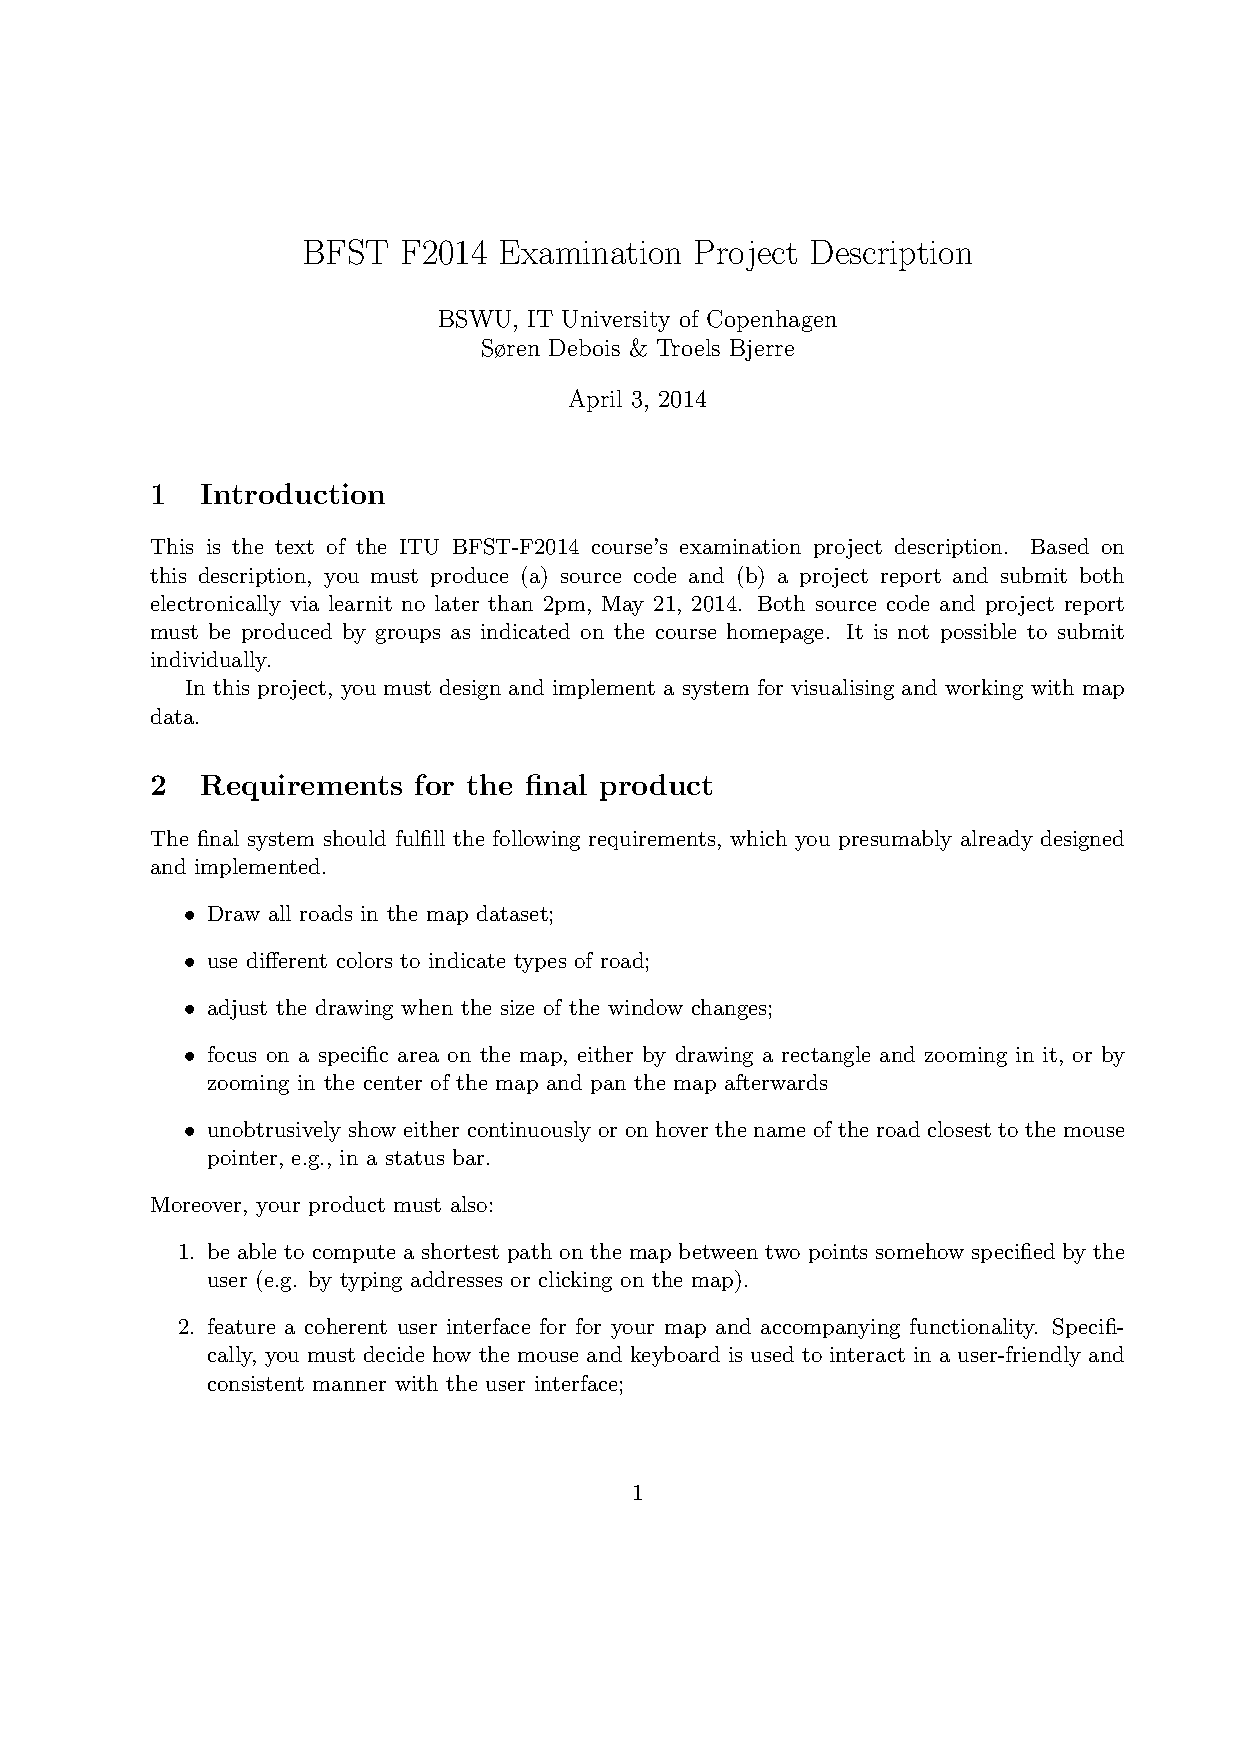
\includepdf[fitpaper,pages={-}]{Bilag/oblikrav}

\section{Brugsvejledning}
\label{sec:Brugervejledning}
Programmet kan køres via den udleverede .jar-fil. Efter start af programmet kan det tage op til 5 sekunder før kortet ses på skærmen.
\begin{table}[h!t]
\centering
	\caption{Tastaturgenveje}
	\begin{tabular}{p{3cm} l l l}
		\hline\hline
		Kommando & Tast & Tast & Tast \\ [0.5ex]
		\hline
		Zoom kortet ind & i & + & num+\\
		Zoom kortet ud & o & - & num-\\
		Returner kortet til startzoomgrad og centrer kortet & r & space & backspace\\
		Bevæg kortet & piletasterne\\
		\hline
	\end{tabular}
\end{table}

\begin{table}[h!t]
\centering
	\caption{Mussemanipulation}
	\begin{tabular}{p{3cm} l l p{5cm}}
		\hline\hline
		Kommando & bruger \\ [0.5ex]
		\hline
		Zoom kortet ind & Rul musehjulet væk fra bruger\\
		Zoom kortet ud & Rul musehjulet hen mod bruger\\
		Zoom kortet ind i markeret område & Højreklik, træk og slip så du har det ønskede udsnit\\
		Returner kortet til startzoomgrad og centrer kortet & Tryk på den midterste museknap\\
		Bevæg kortet & Venstreklik, træk og slip så du har det ønskede udsnit\\
		\hline
	\end{tabular}
\end{table}

\section{Krakdokumentation}
\label{sec:Krakdokumentation}
\label{Introduction to the KRAK roadmap data and associated code}
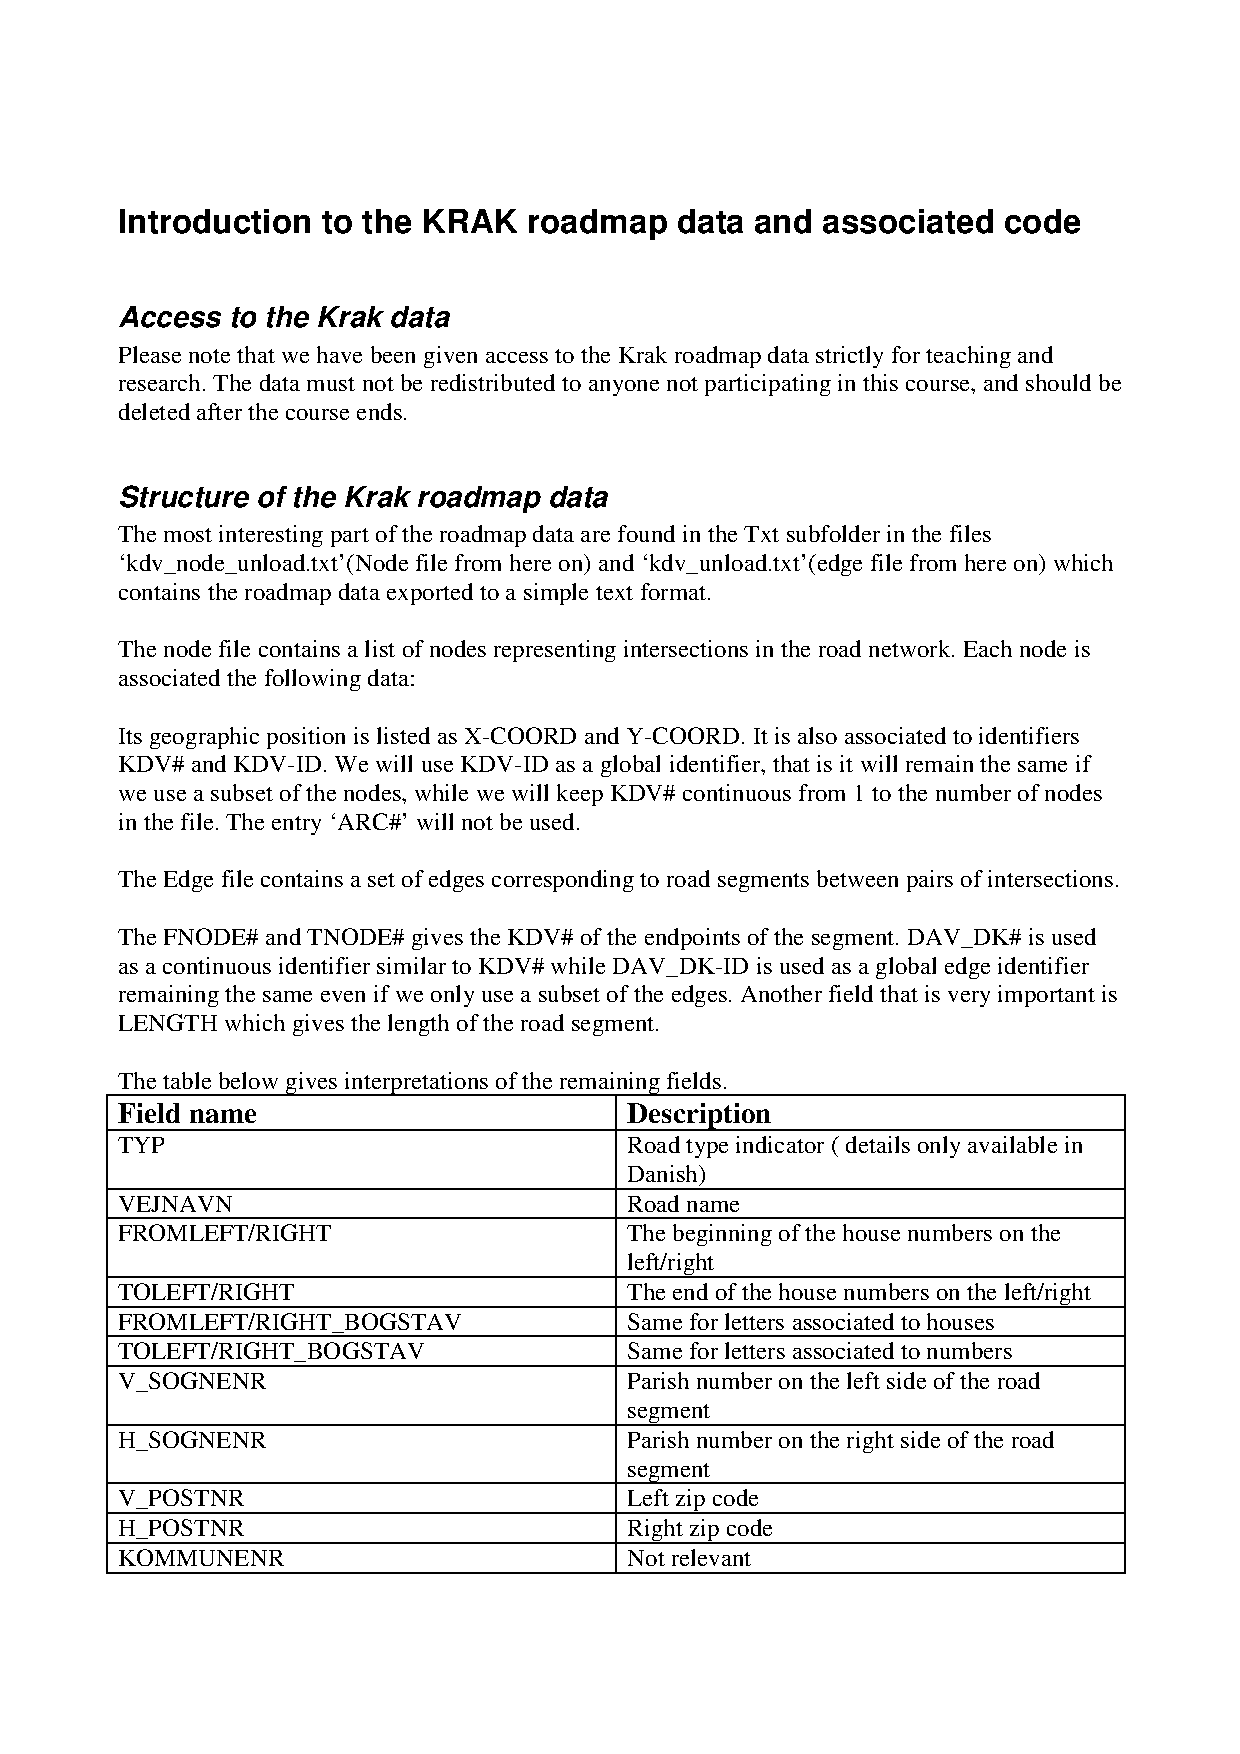
\includepdf[fitpaper,pages={-}]{Bilag/krak1}
\label{Dokumentation KDV}

\includepdf[fitpaper,pages={-}]{Bilag/krak2}

\section{Arbejdslog}
\label{sec:Arbejdslog}
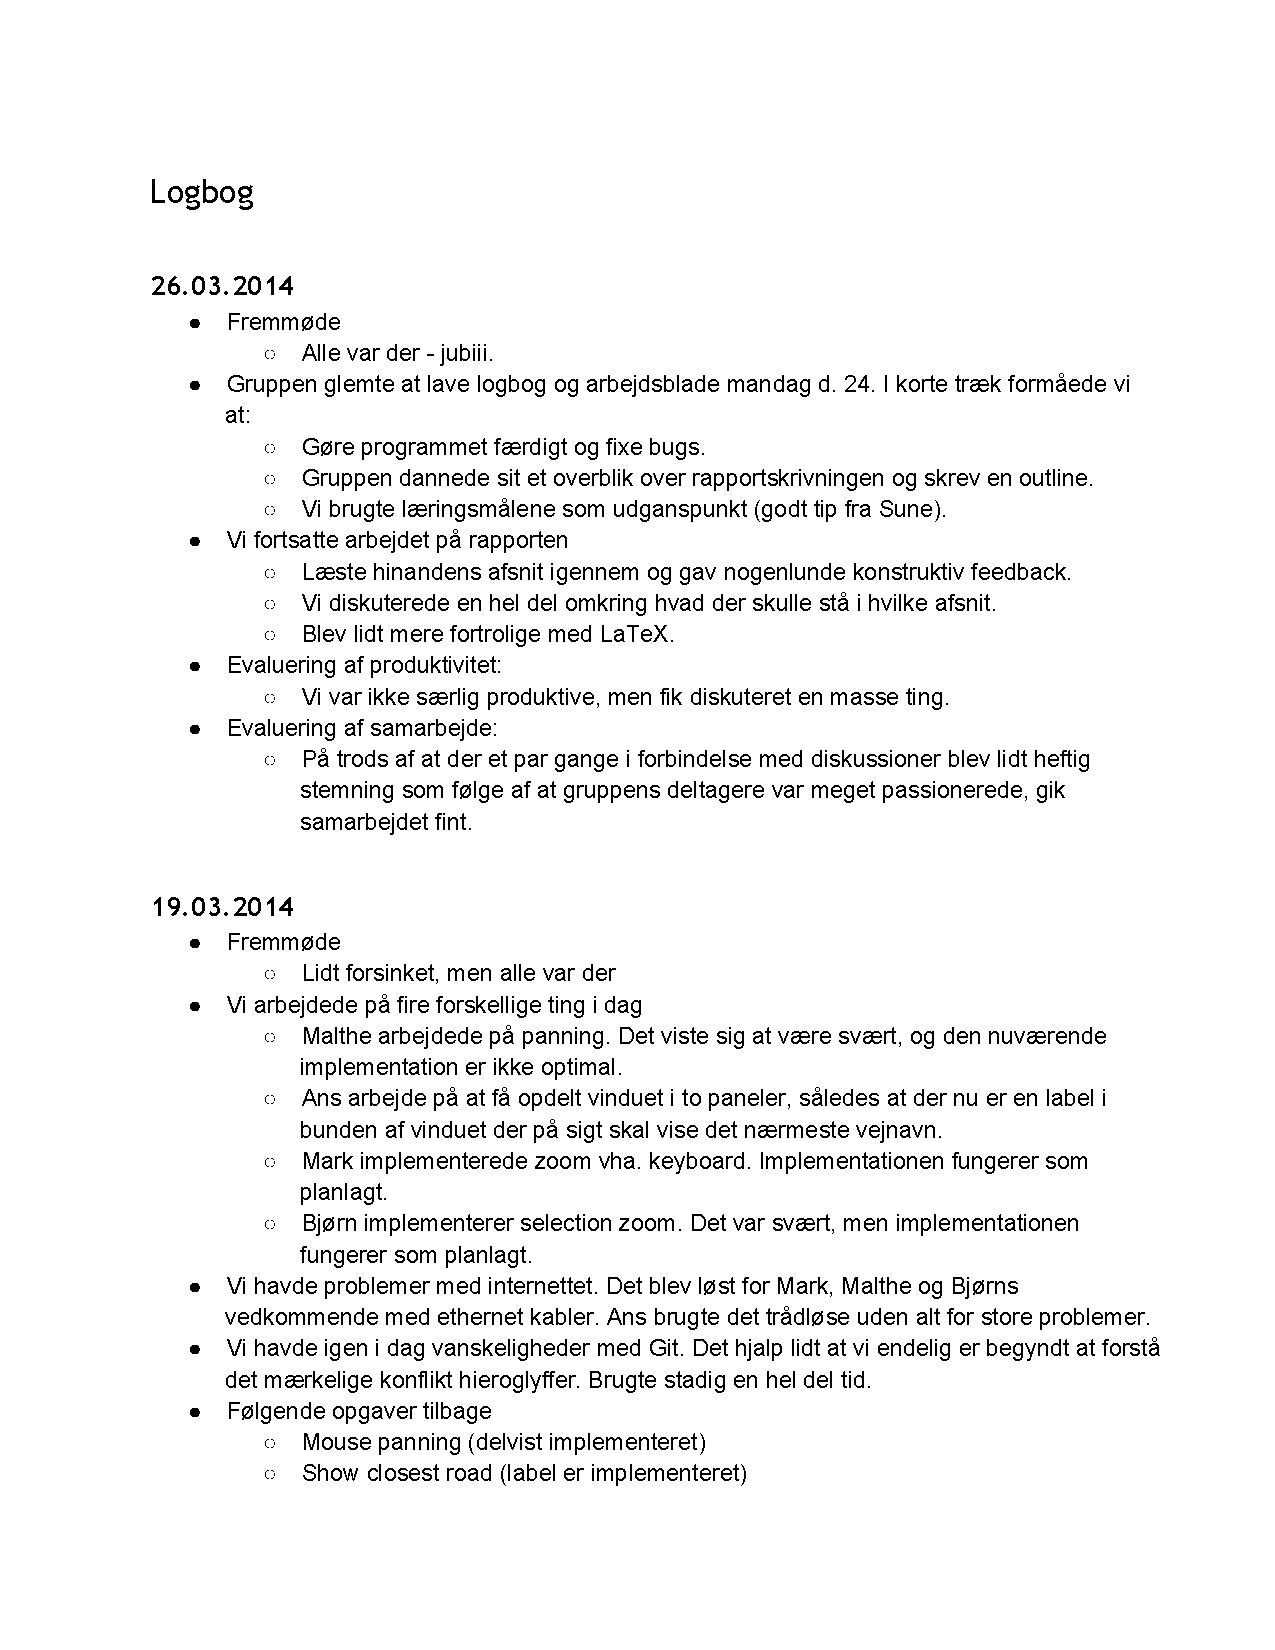
\includepdf[fitpaper,pages={-}]{Bilag/Logbog}

\section{Arbejdsblade}
\label{sec:Arbejdsblade}
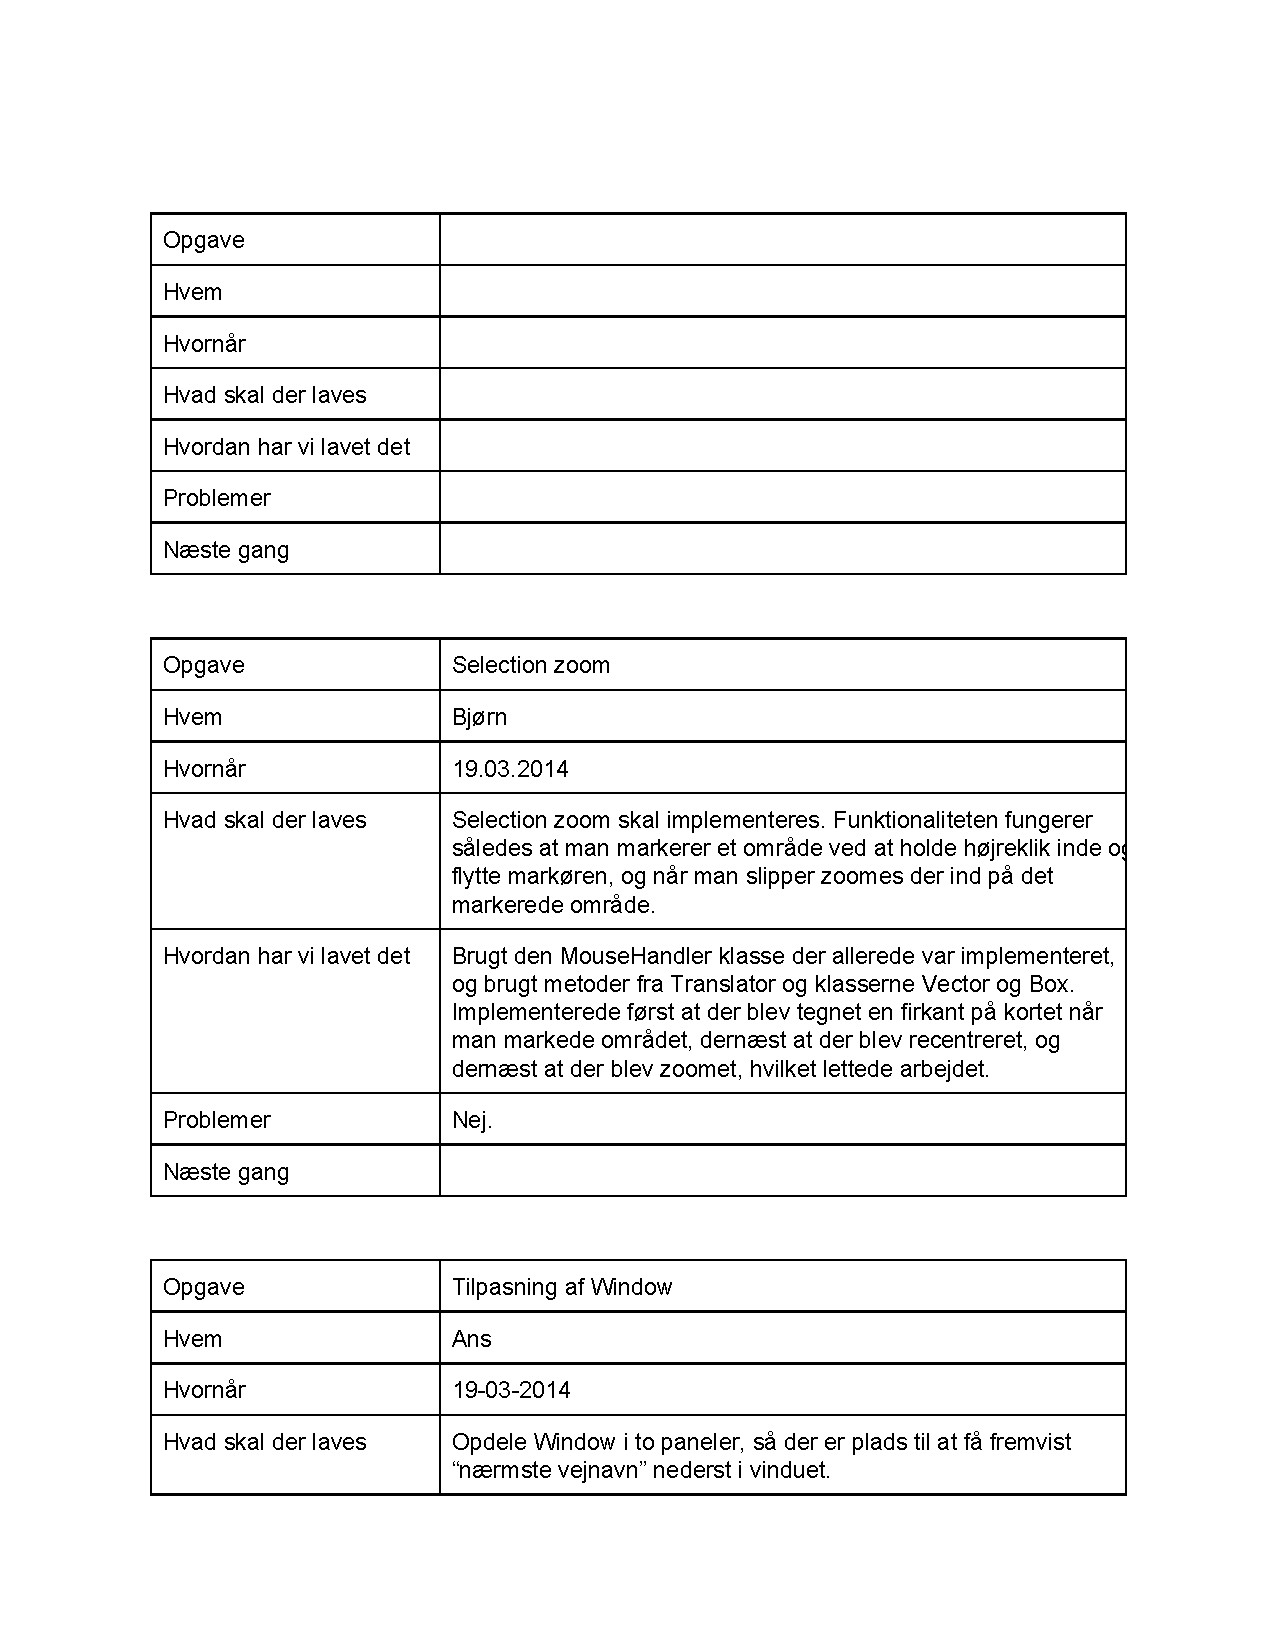
\includepdf[fitpaper,pages={-}]{Bilag/Arbejdsblade}

\section{Samarbejdsaftale}
\label{sec:Samarbejdsaftale}
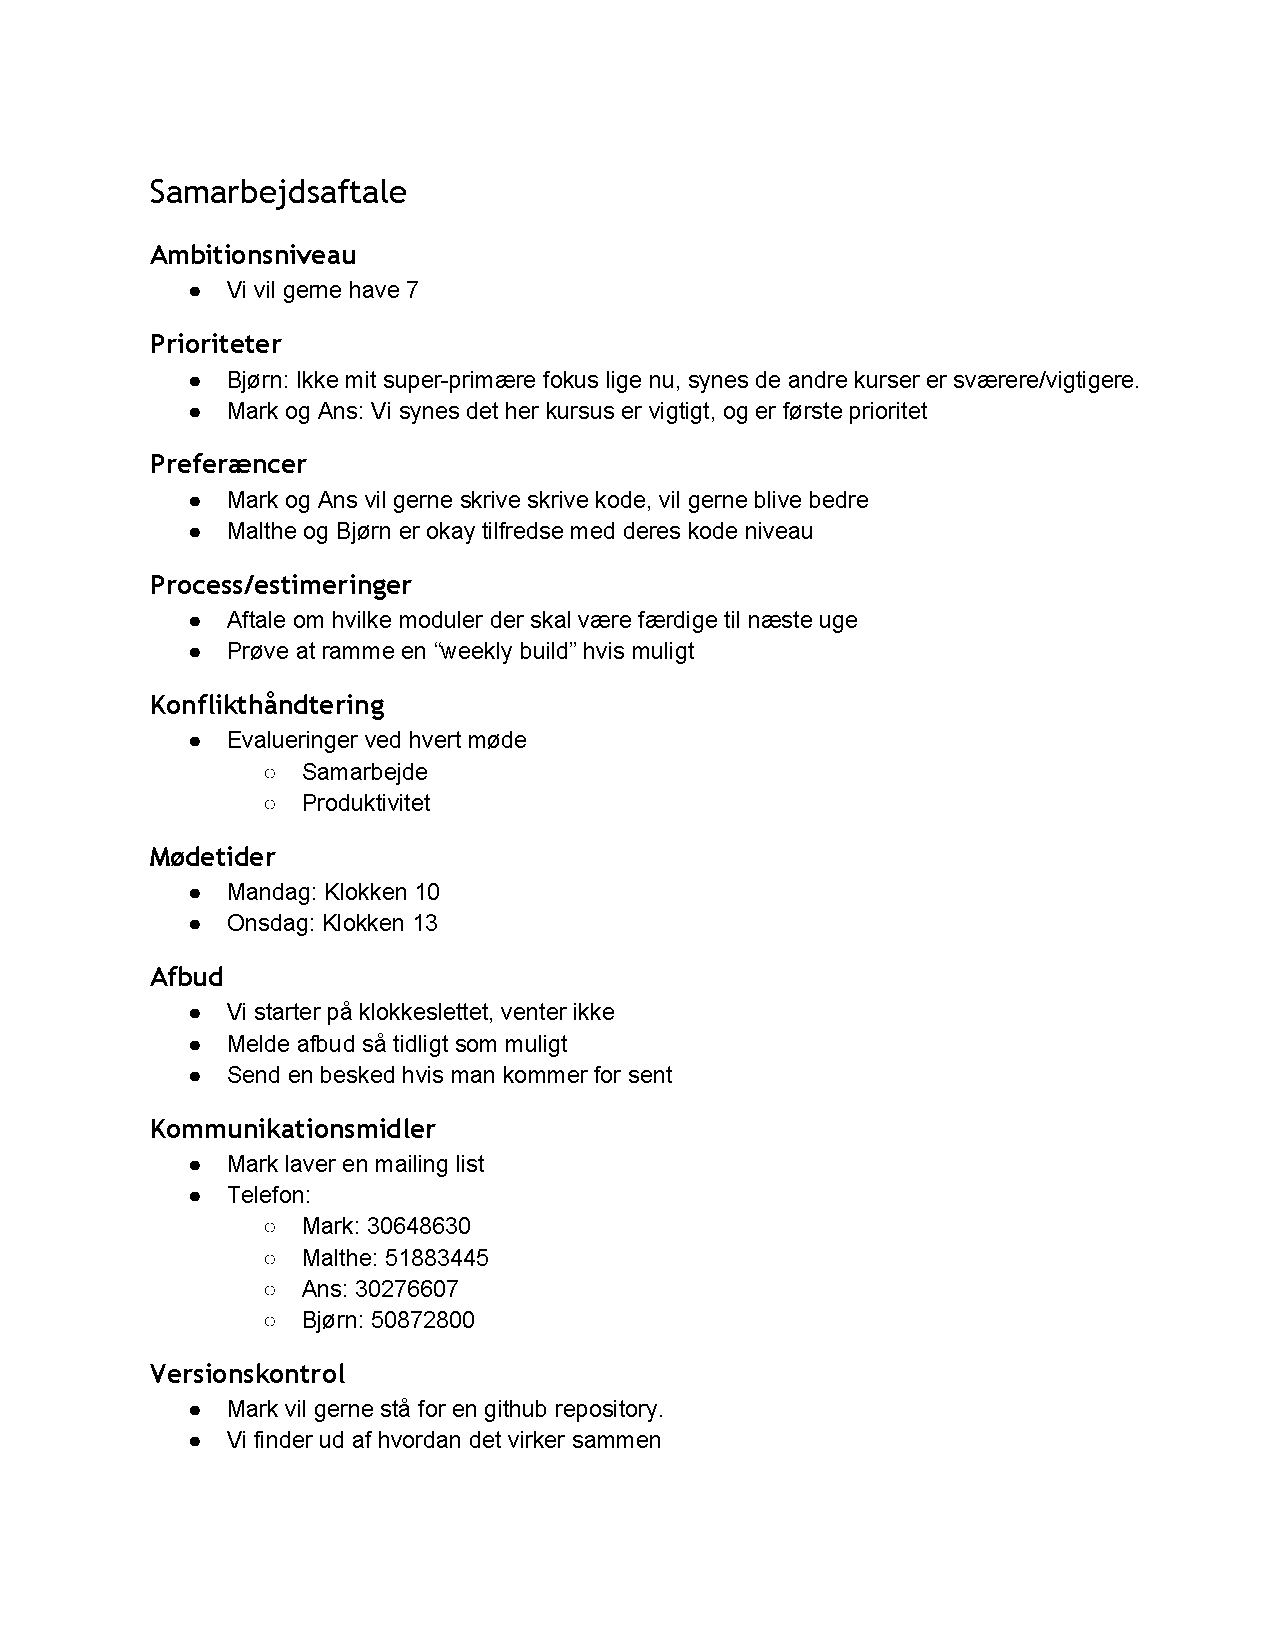
\includepdf[fitpaper,pages={-}]{Bilag/Samarbejdsaftale}


\section{Forventningstabeller}
\label{sec:forventningstabeller}
	\subsection{Vector}
	\newcolumntype{L}{>{\centering\arraybackslash}m{4cm}}

\begin{table}[!h]
	\caption{Vector:Constructor}
	\centering
	\begin{tabular}{L L L}
		\hline\hline
		Input data & Forventet output & Egentligt output \\ [0.5ex]
		\hline
		vec(1,2) & vec(1,2) & vec(1,2) \\
		\hline
	\end{tabular}
\end{table}

\begin{table}[!h]
	\caption{Vector:Set}
	\centering
	\begin{tabular}{L L L}
		\hline\hline
		Input data & Forventet output & Egentligt output \\ [0.5ex]
		\hline
		vec(2,3) & vec(2,3) & vec(2,3) \\
		\hline
	\end{tabular}
\end{table}

\begin{table}[!h]
	\caption{Vector:Copy}
	\centering
	\begin{tabular}{L L L}
		\hline\hline
		Input data & Forventet output & Egentligt output \\ [0.5ex]
		\hline
		vec(1,2) & vec(1,2) & vec(1,2) \\
		\hline
	\end{tabular}
\end{table}

\begin{table}[!h]
	\caption{Vector:Add}
	\centering
	\begin{tabular}{L L L}
		\hline\hline
		Input data & Forventet output & Egentligt output \\ [0.5ex]
		\hline
		vec(1,2)+vec(1,1) & vec(2,3) & vec(2,3)\\
		vec(1,2)+vec(-1,-1) & vec(0,1) & vec(0,1)\\
		vec(1,2)+vec(0,0) & vec(1,2) & vec(1,2)\\
		\hline
	\end{tabular}
\end{table}

\begin{table}[!h]
	\caption{Vector:Subtract}
	\centering
	\begin{tabular}{L L L}
		\hline\hline
		Input data & Forventet output & Egentligt output \\ [0.5ex]
		\hline
		vec(1,2)-vec(1,1) & vec(0,1) & vec(0,1)\\
		vec(1,2)-vec(-1,-1) & vec(-1,-1) & vec(-1,-1)\\
		vec(1,2)-vec(0,0) & vec(1,2) & vec(1,2)\\
		\hline
	\end{tabular}
\end{table}

\begin{table}[!h]
	\caption{Vector:Multiplication}
	\centering
	\begin{tabular}{L L L}
		\hline\hline
		Input data & Forventet output & Egentligt output \\ [0.5ex]
		\hline
		vec(1,2)*2 & vec(2,4) & vec(2,4)\\
		vec(1,2)*0.5 & vec(0.5,1) & vec(0.5,1)\\
		vec(1,2)*1 & vec(1,2) & vec(1,2)\\
		\hline
	\end{tabular}
\end{table}

\begin{table}[!h]
	\caption{Vector:Division}
	\centering
	\begin{tabular}{L L L}
		\hline\hline
		Input data & Forventet output & Egentligt output \\ [0.5ex]
		\hline
		vec(1,2)/0.5 & vec(2,4) & vec(2,4)\\
		vec(1,2)/2 & vec(0.5,1) & vec(0.5,1)\\
		vec(1,2)/1 & vec(1,2) & vec(1,2)\\
		\hline
	\end{tabular}
\end{table}

\begin{table}[!h]
	\caption{Vector:Distance}
	\centering
	\begin{tabular}{L L L}
		\hline\hline
		Input data & Forventet output & Egentligt output \\ [0.5ex]
		\hline
		vec(1,2) to vec(2,3) & $ \sqrt{2} $ & $ \sqrt{2} $\\
		vec(1,2) to vec(0,1) & $ \sqrt{2} $ & $ \sqrt{2} $\\
		vec(1,2) to vec(1,2) & 0 & 0\\
		\hline
	\end{tabular}
\end{table}

\begin{table}[!h]
	\caption{Vector:Translate}
	\centering
	\begin{tabular}{L L L}
		\hline\hline
		Input data & Forventet output & Egentligt output \\ [0.5ex]
		\hline
		vec(1,2) from box(0,0;2,4) to box(0,0;4,8) & vec(2,4) & vec(2,4)\\
		\hline
	\end{tabular}
\end{table}

\begin{table}[!h]
	\caption{Vector:isInside (i box(0,0; 1,1) )}
	\centering
	\begin{tabular}{L L L}
		\hline\hline
		Input data & Forventet output & Egentligt output \\ [0.5ex]
		\hline
		vec(0,0) & true & true\\
		vec(0.5,0.5) & true & true\\
		vec(1,1) & true & true\\
		vec(0,1.01) & false & false\\
		vec(1.01,0) & false & false\\
		vec(1.01,1.01) & false & false\\
		\hline
	\end{tabular}
\end{table}

\begin{table}[!h]
	\caption{Vector:MirrorY}
	\centering
	\begin{tabular}{L L L}
		\hline\hline
		Input data & Forventet output & Egentligt output \\ [0.5ex]
		\hline
		vec(1,2) in box(0,0;1,3) & vec(1,1) & vec(1,1)\\
		\hline
	\end{tabular}
\end{table}

\begin{table}[!h]
	\caption{Vector:Abs}
	\centering
	\begin{tabular}{L L L}
		\hline\hline
		Input data & Forventet output & Egentligt output \\ [0.5ex]
		\hline
		vec(-1,-1) & vec(1,1) & vec(1,1)\\
		\hline
	\end{tabular}
\end{table}

\begin{table}[!h]
	\caption{Vector:Dot}
	\centering
	\begin{tabular}{L L L}
		\hline\hline
		Input data & Forventet output & Egentligt output \\ [0.5ex]
		\hline
		vec(0,0)$\cdot$vec(0,0) & 0 & 0\\
		vec(0,0)$\cdot$vec(1,3) & 0 & 0\\
		vec(0,0)$\cdot$vec(-2,-5) & 0 & 0\\
		vec(0,0)$\cdot$vec(-3,4) & 0 & 0\\
		\hline
		vec(1,3)$\cdot$vec(0,0) & 0 & 0\\
		vec(1,3)$\cdot$vec(1,3) & 10 & 10\\
		vec(1,3)$\cdot$vec(-2,-5) & -17 & -17\\
		vec(1,3)$\cdot$vec(-3,4) & 9 & 9\\
		\hline
		vec(-2,-5)$\cdot$vec(0,0) & 0 & 0\\
		vec(-2,-5)$\cdot$vec(1,3) & -17 & -17\\
		vec(-2,-5)$\cdot$vec(-2,-5) & 29 & 29\\
		vec(-2,-5)$\cdot$vec(-3,4) & -14 & -14\\
		\hline
		vec(-3,4)$\cdot$vec(0,0) & 0 & 0\\
		vec(-3,4)$\cdot$vec(1,3) & 9 & 9\\
		vec(-3,4)$\cdot$vec(-2,-5) & -14 & -14\\
		vec(-3,4)$\cdot$vec(-3,4) & 25 & 25\\
		\hline
	\end{tabular}
\end{table}

\begin{table}[!h]
	\caption{Vector:Cross}
	\centering
	\begin{tabular}{L L L}
		\hline\hline
		Input data & Forventet output & Egentligt output \\ [0.5ex]
		\hline
		vec(0,0)$\times$vec(0,0) & 0 & 0\\
		vec(0,0)$\times$vec(1,3) & 0 & 0\\
		vec(0,0)$\times$vec(-2,-5) & 0 & 0\\
		vec(0,0)$\times$vec(-3,4) & 0 & 0\\
		\hline
		vec(1,3)$\times$vec(0,0) & 0 & 0\\
		vec(1,3)$\times$vec(1,3) & 0 & 0\\
		vec(1,3)$\times$vec(-2,-5) & 1 & 1\\
		vec(1,3)$\times$vec(-3,4) & 13 & 13\\
		\hline
		vec(-2,-5)$\times$vec(0,0) & 0 & 0\\
		vec(-2,-5)$\times$vec(1,3) & -1 & -1\\
		vec(-2,-5)$\times$vec(-2,-5) & 0 & 0\\
		vec(-2,-5)$\times$vec(-3,4) & -23 & -23\\
		\hline
		vec(-3,4)$\times$vec(0,0) & 0 & 0\\
		vec(-3,4)$\times$vec(1,3) & -13 & -13\\
		vec(-3,4)$\times$vec(-2,-5) & 23 & 23\\
		vec(-3,4)$\times$vec(-3,4) & 0 & 0\\
		\hline
	\end{tabular}
\end{table}

\begin{table}[!h]
	\caption{Vector:Mag}
	\centering
	\begin{tabular}{L L L}
		\hline\hline
		Input data & Forventet output & Egentligt output \\ [0.5ex]
		\hline
		vec(0,0) & 0 & 0\\
		vec(1,3)  & $\sqrt{5}$ & $\sqrt{5}$\\
		vec(-2,-5) & $\sqrt{5}$ & $\sqrt{5}$\\
		vec(-3,4) & $\sqrt{5}$ & $\sqrt{5}$\\
		\hline
	\end{tabular}
\end{table}

\begin{table}[!h]
	\caption{Vector:Norm}
	\centering
	\begin{tabular}{L L L}
		\hline\hline
		Input data & Forventet output & Egentligt output \\ [0.5ex]
		\hline
		vec(10,0) & vec(0,1) & vec(0,1)\\
		\hline
	\end{tabular}
\end{table}

\begin{table}[!h]
	\caption{Vector:AngleBetween}
	\centering
	\begin{tabular}{L L L}
		\hline\hline
		Input data & Forventet output & Egentligt output \\ [0.5ex]
		\hline
		vec(1,2)$\angle$vec(1,2) & 0 & 0\\
		vec(1,2)$\angle$vec(2,-1) & $-\pi/2$ & $-\pi/2$\\
		vec(1,2)$\angle$vec(-1,-2) & $\pi$ & $\pi$\\
		vec(1,2)$\angle$vec(-2,1) & $\pi/2$ & $\pi/2$\\
		\hline
	\end{tabular}
\end{table}

\begin{table}[!h]
	\caption{Vector:Equals}
	\centering
	\begin{tabular}{L L L}
		\hline\hline
		Input data & Forventet output & Egentligt output \\ [0.5ex]
		\hline
		vec(7,21) og vec(7,21) & true & true\\
		vec(7,21) og vec(21,7) & false & false\\
		vec(7,21) og vec(0,-90) & false & false\\
		\hline
	\end{tabular}
\end{table}
\newpage
	\subsection{Box}
	\newcolumntype{L}{>{\centering\arraybackslash}m{4cm}}

\subsection{Box}

\begin{table}[ht]
	\caption{Box:Constructor}
	\centering
	\begin{tabular}{L L L}
		\hline\hline
		Input data & Forventet output & Egentligt output \\ [0.5ex]
		\hline
		vec(1,2) og vec(3,4) & box(1,2;3,4) & box(1,2;3,4)\\
		\hline
	\end{tabular}
\end{table}

\begin{table}[ht]
	\caption{Box:Dimensions}
	\centering
	\begin{tabular}{L L L}
		\hline\hline
		Input data & Forventet output & Egentligt output \\ [0.5ex]
		\hline
		box(1,2;3,4) & vec(2,2) & vec(2,2)\\
		\hline
	\end{tabular}
\end{table}

\begin{table}[ht]
	\caption{Box:RelativeToAbsolute}
	\centering
	\begin{tabular}{L L L}
		\hline\hline
		Input data & Forventet output & Egentligt output \\ [0.5ex]
		\hline
		vec(0.5,0.5) i box(1,2;3,4) & vec(2,3) & vec(2,3)\\
		\hline
	\end{tabular}
\end{table}

\begin{table}[ht]
	\caption{Box:Ratio}
	\centering
	\begin{tabular}{L L L}
		\hline\hline
		Input data & Forventet output & Egentligt output \\ [0.5ex]
		\hline
		box(1,2;3,4) & vec(1,1) & vec(1,1)\\
		box(0,0;2,1) & vec(1,0.5) & vec(1,0.5)\\
		box(0,0;1,2) & vec(0.5,1) & vec(0.5,1)\\
		\hline
	\end{tabular}
\end{table}

\begin{table}[ht]
	\caption{Box:Scale}
	\centering
	\begin{tabular}{L L L}
		\hline\hline
		Input data & Forventet output & Egentligt output \\ [0.5ex]
		\hline
		box(1,2;3,4)*2 & box(0,1;4,5) & box(0,1;4,5)\\
		\hline
	\end{tabular}
\end{table}

\begin{table}[ht]
	\caption{Box:FlipX}
	\centering
	\begin{tabular}{L L L}
		\hline\hline
		Input data & Forventet output & Egentligt output \\ [0.5ex]
		\hline
		box(11,0;-3,0) & box(-3,0;11,0) & box(-3,0;11,0)\\
		\hline
	\end{tabular}
\end{table}

\begin{table}[ht]
	\caption{Box:FlipY}
	\centering
	\begin{tabular}{L L L}
		\hline\hline
		Input data & Forventet output & Egentligt output \\ [0.5ex]
		\hline
		box(0,11;0,-3) & box(0,-3;0,11) & box(0,-3;0,11)\\
		\hline
	\end{tabular}
\end{table}

\begin{table}[ht]
	\caption{BoxProperCorners}
	\centering
	\begin{tabular}{L L L}
		\hline\hline
		Input data & Forventet output & Egentligt output \\ [0.5ex]
		\hline
		box(51,-10;0,80) & box(0,-10;51,80) & box(0,-10;51,80)\\
		\hline
	\end{tabular}
\end{table}


\end{document}